\documentclass[11pt,letterpaper]{article}

%\usepackage[latin1]{inputenc} 
\usepackage[utf8]{inputenc}
\usepackage[cyr]{aeguill}
\usepackage[colorlinks=true]{hyperref}
\usepackage{textpos}
\usepackage{graphicx}
\usepackage[french]{babel}
\usepackage{color}
\usepackage{array}
\usepackage{enumerate}
\usepackage{fancyhdr}
\usepackage{lastpage}
\usepackage{amsmath}
\usepackage{amssymb}
\usepackage{epstopdf}
\usepackage{mathrsfs}
\usepackage{float}
\usepackage{multicol}
\usepackage{caption}
\usepackage{subcaption}
\usepackage{siunitx}
\addto\captionsfrench{\def\tablename{Tableau}}

%-----------------------------------------------------------------%
% Definitions
\newcommand{\session}{Hiver 2022}
\newcommand{\firstauthor}{Yoan \textbf{Fournier}}
\newcommand{\firstregistrationnumber}{1958736}
\newcommand{\secondauthor}{Victor \textbf{Gaudreau-Blouin}}
\newcommand{\secondregistrationnumber}{1958297}
\newcommand{\reportnumber}{}
\newcommand{\firsttitle}{Analyse énergétique d'un processeur vectoriel pour des calculs de DNN}
\newcommand{\secondtitle}{Rapport intermédiaire}
%-----------------------------------------------------------------%



\oddsidemargin 0pt
\topmargin 0pt
\textwidth 6.5in
\textheight 8.1in

\setlength{\parskip}{1em}

\definecolor{bleu_poly}{RGB}{65,170,230}
\definecolor{vert_poly}{RGB}{140,200,60}
\definecolor{orange_poly}{RGB}{250,150,30}
\definecolor{rouge_poly}{RGB}{185,30,50}
\definecolor{gris_poly}{RGB}{166,168,171}


\title{\vspace{-2.5cm} \noindent\makebox[\linewidth]{\color{rouge_poly}{\rule{\textwidth}{1.5pt}}}
        \begin{center}
        \begin{tabular}{m{6.5cm}m{6cm}}
        \textbf{ \huge Projet \reportnumber}  & 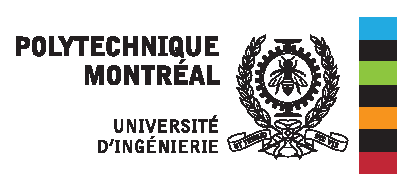
\includegraphics[width=0.4\textwidth]{Polytechnique_signature-CMYK-droite_FR.eps}
        \end{tabular}
        \end{center}
        \noindent\makebox[\linewidth]{\color{rouge_poly}{\rule{\textwidth}{1.5pt}}}
        \\ \  \\
        \Huge \firsttitle \\ \secondtitle  
        \\ \ \\
        \LARGE ELE6307 - Machines neuronales : architectures et applications
        }

\author{\session \\ Département de génie électrique \\ École Polytechnique de Montréal} 

\date{Dernière mise à jour: \today}

\pagestyle{fancy}

\lfoot{\session}
\cfoot{ELE6307 - Machines neuronales : architectures et applications}
\rfoot{\thepage/\pageref{LastPage}}
\chead{}
\lhead{\emph{Projet -- \firstauthor  \, (\firstregistrationnumber)/\secondauthor\,  (\secondregistrationnumber)}}
\rhead{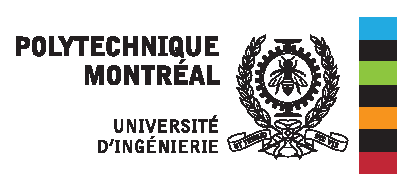
\includegraphics[width=2.5cm]{Polytechnique_signature-CMYK-droite_FR.eps}}
\renewcommand{\headrulewidth}{0.4pt}
\renewcommand{\footrulewidth}{0.4pt} 
\setlength{\headheight}{45pt}


\graphicspath{{fig/}}


\newcommand{\vb}[1]{\mathbf{#1}}
\newcommand{\bs}[1]{\boldsymbol{#1}}


%-----------------------------------------------------------------%
% SOF
\begin{document}
\maketitle
\noindent\makebox[\linewidth]{\color{rouge_poly}{\rule{\textwidth}{1.5pt}}} 


\noindent \LARGE \firstauthor  \hfill \firstregistrationnumber


\noindent \LARGE \secondauthor \hfill \secondregistrationnumber


\noindent\makebox[\linewidth]{\color{rouge_poly}{\rule{\textwidth}{1.5pt}}}


\newpage
\normalsize

\section*{Introduction}
    \begin{multicols}{2}
    Afin de modéliser l'efficacité énergétique du coprocesseur vectoriel ARA, le simulateur Timeloop a été 
    utilisé. Ce simulateur utilise une structure hiérarchique pour modéliser une architecture. Une structure
    détaillant le problème à résoudre par l'architecture est aussi spécifiée. La commande \textit{timeloop-mapper}
    permet ensuite de trouver automatiquement la correspondance idéale du problème sur l'architecture matérielle.

    L'architecture simplifiée de ARA, comme mentionnée dans la proposition du projet, peut se modéliser en termes de 
    \textit{Lanes}. Chaque \textit{Lanes} à sa plus simple expression consiste en une banque de 8 registres ainsi qu'une
    unité arithmétique capable d'effectuer des multiplications et des additions. Bien que sur ARA, l'unité d'addition 
    est séparée de l'unité de multiplication, les deux unités peuvent fonctionner durant le même cycle sur des données
    indépendantes. Dans le cadre de la modélisation, on simplifie en utilisant la structure \textit{intmac} fournie par
    l'outil Timeloop-Accelergy. Nous considérons que la différence causée par cette simplification est minimale. En effet,
    les opérations dans une Lane sont pipelinées et les opérations de multiplication et addition peuvent être exécutées en même temps.
    La seule différence principale est la latence causée par le pipelinage des opérations. Cependant, ce n'est pas une métrique
    de performance étudiée dans le cadre de ce projet.

    L'architecture utilisée est présentée à la figure \ref{fig:arch}. On y observe une mémoire DRAM principale reliée à 
    la mémoire cache L1 de 64 KB. La cache L1 est reliée à un nombre paramétrable de \textit{Lanes}. 
    Chaque \text{Lane} comporte sa banque de 8 registres et son unité de \text{multiply-accumulate}.

    \begin{figure}[H]
        \centering
        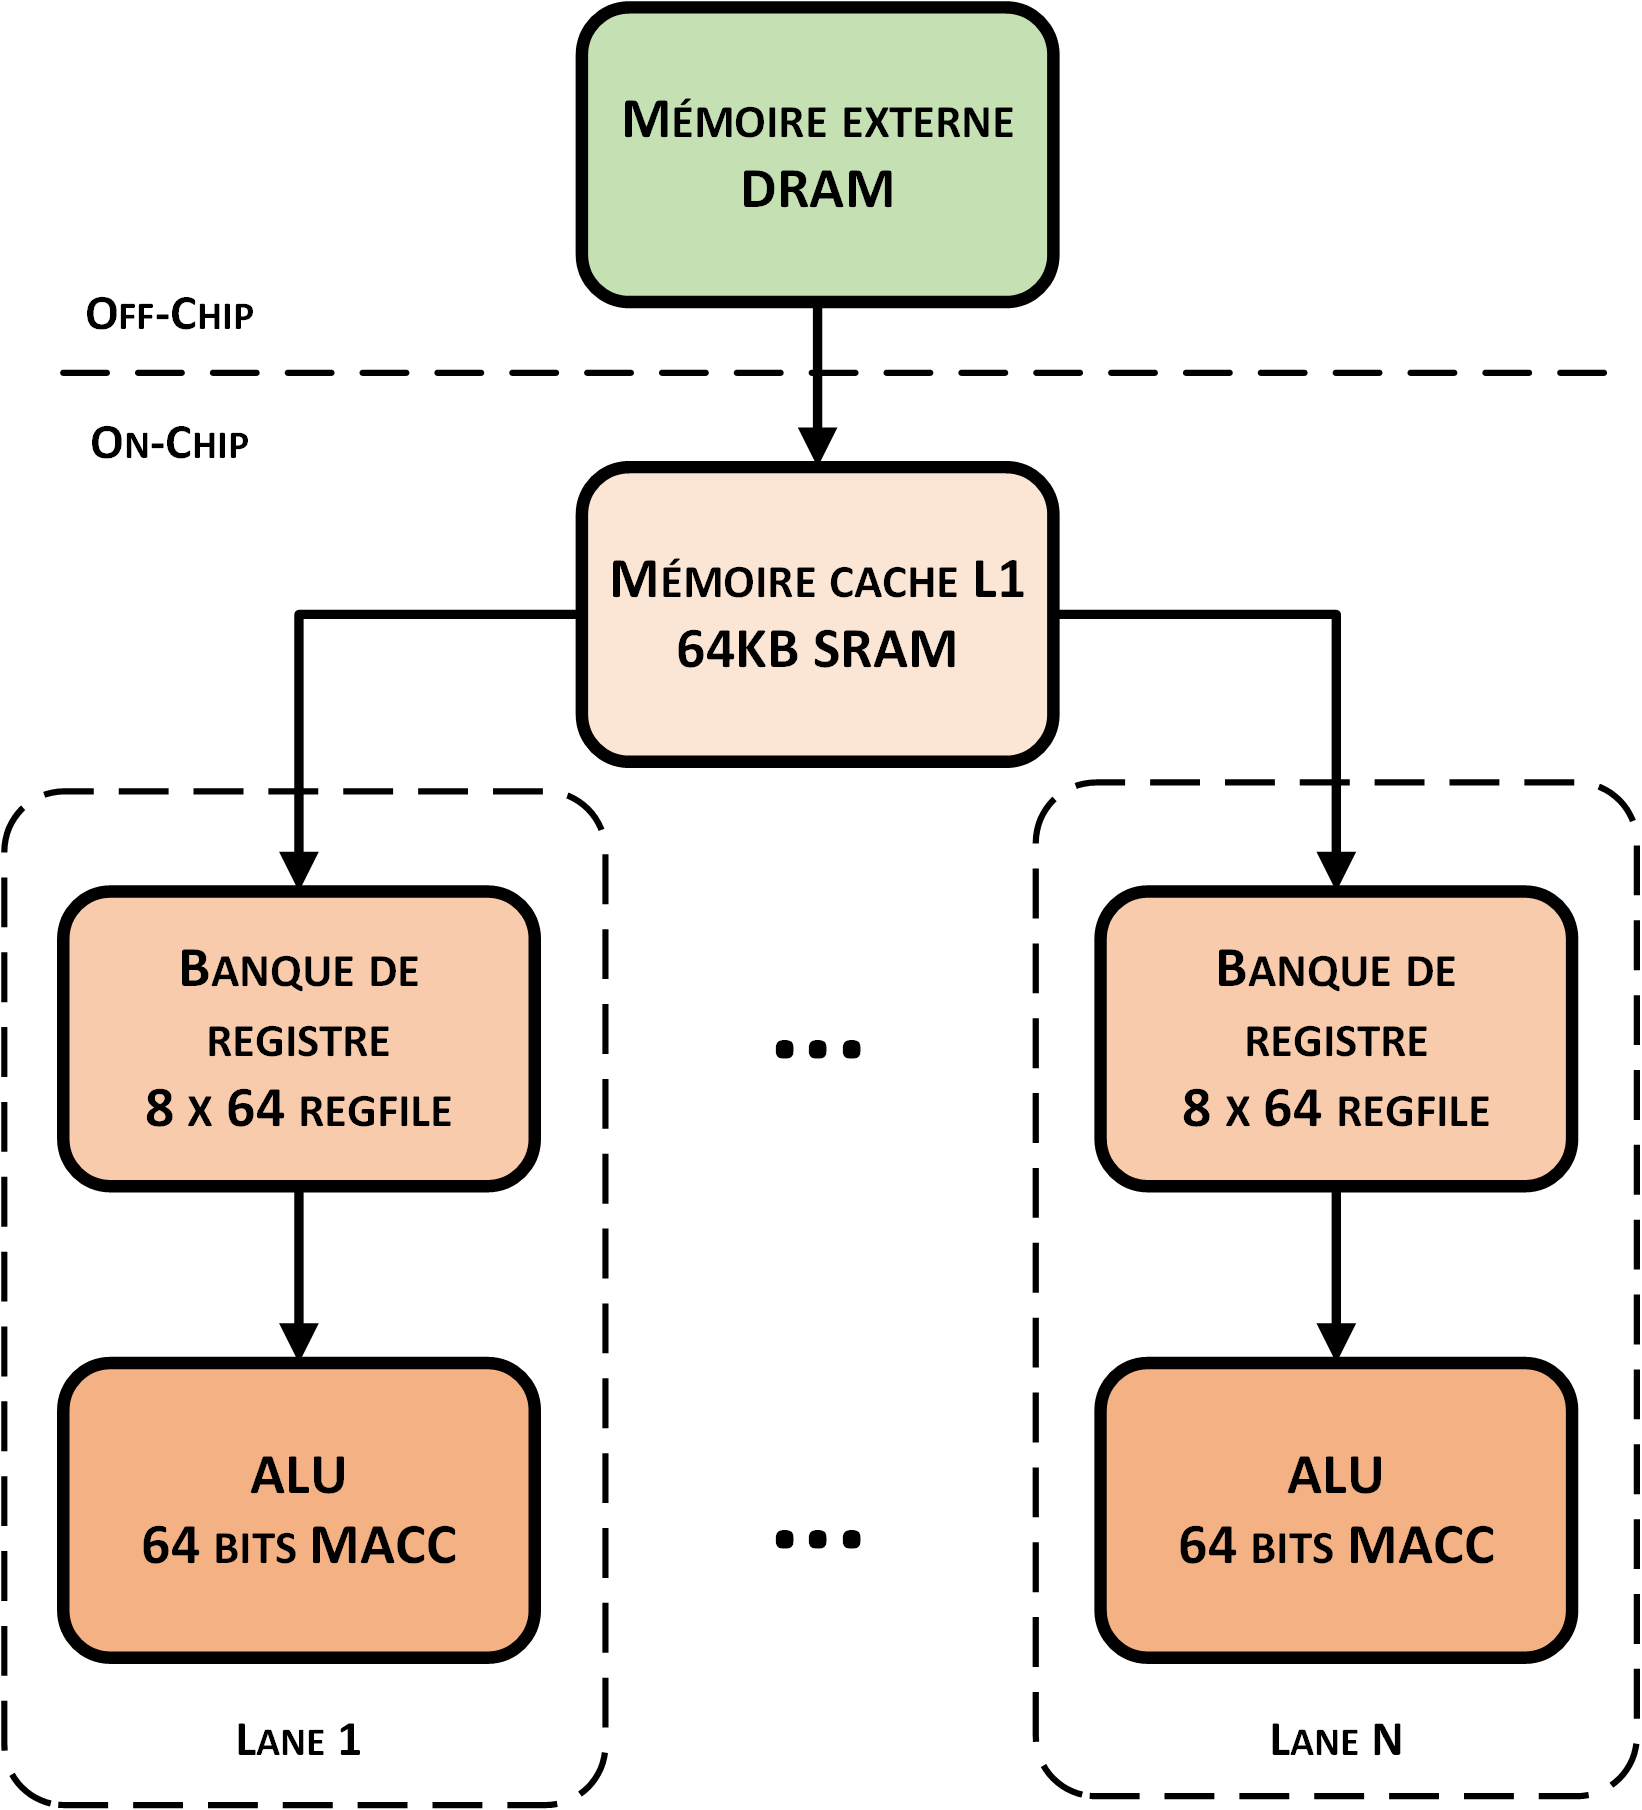
\includegraphics[width=\linewidth]{arch_visio.png}
        \caption{Architecture de ARA sur Timeloop}
        \label{fig:arch}
    \end{figure}

    Afin d'étudier la performance de l'architecture en fonction du nombre de \textit{Lanes}, le problème utilisé est la première 
    couche convolutionnelle du modèle VGG16. Cette couche comporte 64 filtres avec un \textit{kernel} de $3\times3$. L'entrée de la couche
    est une image de dimension $224\times224\times3$.  

    \end{multicols}


\pagebreak
\section*{Résultats}
    \begin{multicols}{2}

    On montre ci-dessous les résultats d'aire, d'énergie, de nombre de cycles, d'utilisation et de performance 
    de ARA en fonction du nombre de \textit{Lanes} utilisé. Certains résultats sont attendus, comme la relation 
    linéaire entre le nombre de \textit{Lanes} et le nombre de cycles. En effet, en doublant le nombre de \textit{Lanes}, 
    il est normal de s'attendre à effectuer la tâche en la moitié du temps, pour autant que ces tâches sont indépendantes.
    Une certaine non-linéarité est observée pour les cas de 8 et 16 \textit{Lanes}, mais ceci est dû à l'utilisation 
    non optimale des ressources disponibles, comme on peut le constater sur le graphique d'utilisation. La technologie 
    22 nm tombe à 55 \% d'utilisation à 16 \textit{Lanes}, alors que la technologie 45 nm atteint une utilisation un peu plus 
    haute, à 75 \%, mais à partir de 8 \textit{Lanes}.

    L'aire utilisée croît de manière linéaire. Une particularité à noter est que la différence d'aire sur la technologie 
    22 nm est négligeable, parce que la cache occupe une très grande proportion de l'espace total. 
    Le graphique d'énergie n'est pas aussi direct. On peut noter une tendance descendante dans le coût énergétique total 
    en augmentant le nombre de \textit{Lanes}, mais la courbe n'est pas exactement logarithmique. Ceci est dû en partie à 
    la façon que l'assignation (\textit{mapping}) du circuit est réalisée par Timeloop. Comme le problème d'assignation
    est complexe, il n'est pas garanti de donner la solution optimale pour un ou plusieurs critères. Nous avons la liberté
    de contraindre son espace de recherche pour accélérer la recherche, mais en baissant la probabilité de trouver la 
    solution optimale. Il est donc possible que la solution optimale suive une courbe plus linéaire et surtout décroissante
    sur tout son intervalle. Un point intéressant à noter est que la technologie 45 nm semble avoir une amélioration moins 
    grande que 22 nm, avec 1.5 \% de différence entre l'énergie d'une \textit{Lane} et celle à 16 \textit{Lanes}, versus 
    8.9 \% entre sa consommation maximale et minimale. Finalement, le graphe de performance illustre la combinaison de tous 
    ces facteurs. Ce graphe est obtenu avec la formule $$\text{GFLOP/J} = \frac{\%utilization \times \#cycles \times \#lanes}{E_{tot}}$$.
    On observe une tendance croissante semblant logarithmique. Encore une fois, on peut constater que la technologie 22nm 
    a une meilleure croissance de performance relative, avec 8.5 \% versus 1.5 \% pour 45 nm. De plus, on observe que la 
    performance de la technologie 22 nm avec une seule \textit{Lane} est très supérieure à la meilleure performance de la 
    technologie 45 nm. Ceci nous indique que bien qu'on puisse observer des augmentations de performance en augmentant le nombre
    de \textit{Lanes}, le plus grand facteur est la technologie utilisée.
        
    \begin{figure}[H]
        \centering
        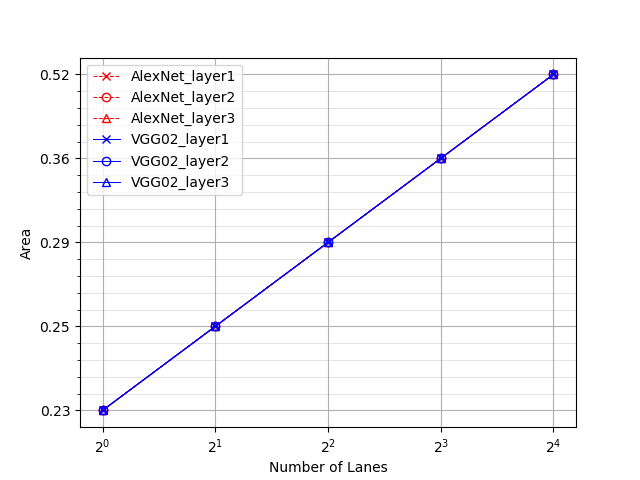
\includegraphics[width=\linewidth]{area.png}
        \caption{Aire de ARA en fonction du nombre de \textit{Lanes} pour la couche 1 de VGG16}
        \label{fig:area}
    \end{figure}
    \begin{figure}[H]
        \centering
        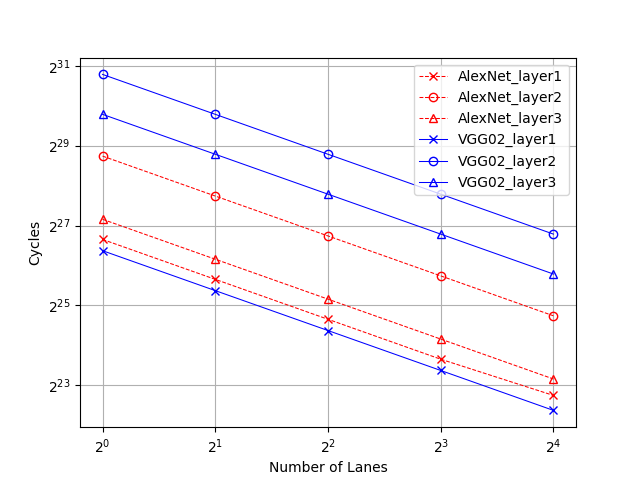
\includegraphics[width=\linewidth]{cycles.png}
        \caption{Cycles de ARA en fonction du nombre de \textit{Lanes} pour la couche 1 de VGG16}
        \label{fig:cycles}
    \end{figure}
    \begin{figure}[H]
        \centering
        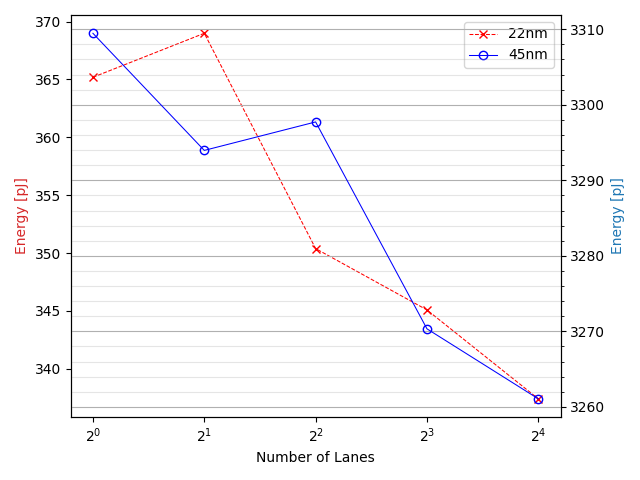
\includegraphics[width=\linewidth]{energy.png}
        \caption{Énergie de ARA en fonction du nombre de \textit{Lanes} pour la couche 1 de VGG16}
        \label{fig:energy}
    \end{figure}
    \begin{figure}[H]
        \centering
        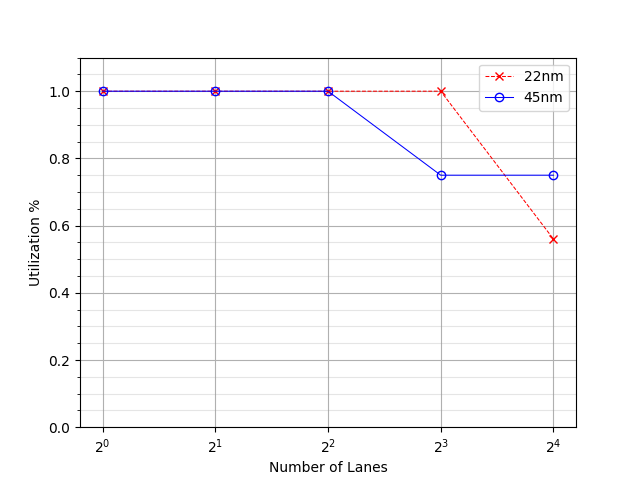
\includegraphics[width=\linewidth]{utilization.png}
        \caption{Utilisation de ARA en fonction du nombre de \textit{Lanes} pour la couche 1 de VGG16}
        \label{fig:utilization}
    \end{figure}
    \begin{figure}[H]
        \centering
        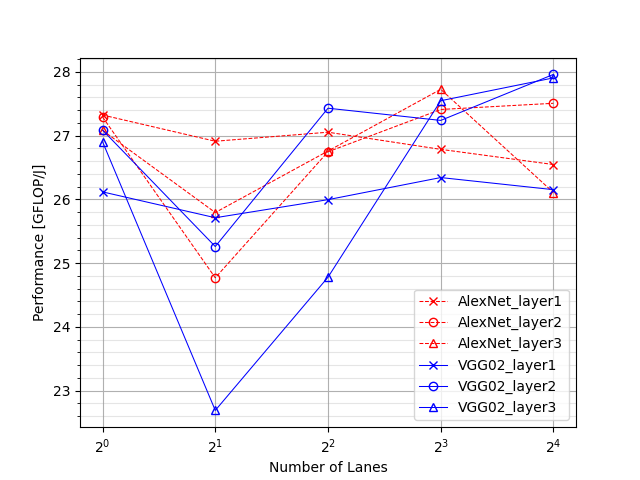
\includegraphics[width=\linewidth]{performance.png}
        \caption{Performance de ARA en GFLOP/J en fonction du nombre de \textit{Lanes} pour la couche 1 de VGG16}
        \label{fig:performance}
    \end{figure}
    
    \end{multicols}

\pagebreak
\section*{Suite du projet}
    %TODO: Rappel des résultats obtenus

    \begin{multicols}{2}
        
    \noindent Pour le rapport final du projet, les aspects suivants seront étudiés plus en détail :
    \begin{enumerate}
        \item \textbf{Utilisation des PE pour 8 et 16 \text{Lanes} :}
            Dans les résultats, on observe que l'allocation n'est pas optimale pour 8 et 16 \textit{Lanes}.
            L'utilisation des PE n'est pas de 100\%. Il serait intéressant de voir si cela est causé par une 
            recherche pas assez exhaustive des allocations ou si une allocation optimale est tout simplement 
            impossible. Le rapport final cherchera à optimiser les paramètres de \textit{timeloop-mapper} afin
            de tenter de converger vers de meilleures solutions.
        \item \textbf{Étudier les allocations optimales :}
            Ce présent rapport ne présente pas l'allocation optimale trouvée par Timeloop. Le rapport finale 
            présentera plus en détail cette allocation. En effet, le problème est automatiquement partitionné
            par Timeloop afin d'optimiser au maximum l'énergie consommée par l'architecture. Souvent cette métrique
            s'optimise en essayant de réduire au maximum les accès mémoires et d'optimiser la localité des données.
            L'analyse les allocations effectuées par Timeloop permettra de mieux comprendre l'approche optimale a utilisée
            et permettra de déceler les goulots d'étranglement dans l'architecture proposée.
        \item \textbf{Tester l'impact des paramètres du problème :} 
            Le seul problème étudié dans le cadre de ce rapport intermédiaire est la couche 1 du modèle VGG16.
            Afin d'avoir une meilleure idée de la performance de l'architecture, il serait intéressant de faire
            varier les paramètres du problème comme le \text{kernel} ou la taille des tenseurs d'entrée. On pourrait
            y observer une diminution de l'utilité d'avoir plusieurs \text{Lanes} lorsque les problèmes sont plus petits
            puisqu'il devient plus difficile de paralléliser les calculs.
    \end{enumerate}
    \end{multicols}

\end{document} 
%-----------------------------------------------------------------%
% EOF